%!TEX root = /Users/louis/Documents/PhD/Deliverables/ProgressReport/pr.tex
\subsection{Locating Examples of Evolution}
\label{sub:examples}
In my qualifying dissertation, I identified the need to categorise the ways in which MDE development artefacts evolve over time. The categorisation would be used to provide requirements for developing structures and processes for evolutionary changes in the context of model-driven engineering.

A study of example data (existing MDE projects containing evolution) was proposed to produce this categorisation. Work has progressed by defining requirements for example MDE projects for the study. Existing MDE projects were located and analysed against the requirements. Finally, the most suitable candidate projects were selected. As discussed in Section \ref{sub:analysis_of_existing_techniques}, the selected projects have been used to analyse existing techniques for managing evolution in MDE.

\subsubsection{Requirements} % (fold)
\label{ssub:requirements}
In Section \ref{sub:elaboration}, two categories of evolutionary change were identified: co-evolution and synchronisation. I want to study both. Consequently, requirements are partitioned into three types: those necessary for studying each of the two categories of evolutionary change, and common requirements (applicable to both categories of evolutionary change).

\paragraph{Common requirements}
Every candidate project needs to use some aspect of MDE, such as metamodelling or model transformation (requirement R1). In addition, each candidate project needs to provide historical information to trace the evolution of development artefacts (R2). For example, several versions of the project are needed perhaps in a source code management system. Finally, a candidate project needs to have undergone a number of significant changes\footnote{This is deliberately vague. Further details are given in Section \ref{ssub:project_selection}.} (R3).

\paragraph{Co-evolution requirements}
A candidate project for the study of co-evolution needs to define a metamodel and some changes to that metamodel (R4). In the projects considered, the metamodel changes took the form of either another version of the metamodel, or a history (which recorded each of the steps used to produce the adapted metamodel).

A candidate project also needs to provide example instances of models before and after each migration activity (R5).

Ideally, a candidate project should include more than one consecutive metamodel adaptation, so as to represent the way in which the same development artefacts continue to evolve over time (optional requirement O1).

\paragraph{Synchronisation requirements}
A candidate project for the study of synchronisation needs to define a model-to-model transformation (R6).

Furthermore, a candidate project has to include many examples of source and target models for that transformation (R7).

Crucially, a candidate project needs to provide many examples of the kinds of change (to either source or target model) that cause inconsistency between the models (R8). 

Ideally, a candidate project should also include transformation chains (more than one model-to-model transformation, executed sequentially) (O2). Chains of transformations are prescribed by the MDA guidelines \cite{kleppe03mda}.

% subsubsection requirements (end)

\subsubsection{Project Selection} % (fold)
\label{ssub:project_selection}
Eight candidates were considered for the study. Table \ref{tab:candidates} shows which of the requirements are fulfilled by each of the candidates. Each candidate is now discussed in turn.

\begin{table}
	\caption{Candidates for study of evolution in existing MDE projects}
	\centering
	\begin{tabular}{|c||c|c|c||c|c|c||c|c|c|c|}
		\hline
		\multirow{3}{*}{Name} & \multicolumn{10}{|c|}{Requirements} \\
		\cline{2-11}
		          & \multicolumn{3}{|c||}{Common} & \multicolumn{3}{|c||}{Co-evolution} & \multicolumn{4}{|c|}{Synchronisation} \\
		\cline{2-11}
		          & R1 & R2 & R3 & R4 & R5 & O1 & R6 & R7 & R8 & O2 \\
		\hline
		GSN       & x  &    &    & x  &    &    &    &    &    &    \\
		\hline
		OMG       & x  &    &    & x  &    &    & x  &    &    &    \\
		\hline
		Zoos      & x  & x  &    & x  &    &    &    &    &    &    \\
		\hline
		MDT       & x  & x  &    & x  &    & x  &    &    &    &    \\
		\hline
		MODELPLEX & x  & x  & x  & x  &    & x  & x  & x  &    &    \\
		\hline
		FPTC      & x  & x  & x  & x  & x  &    &    &    &    &    \\
		\hline
		xText     & x  & x  & x  & x  & x  & x  & x  & x  &    & x  \\
		\hline
		GMF       & x  & x  & x  & x  & x  & x  & x  & x  &    & x  \\
		\hline
	\end{tabular}
	\label{tab:candidates}
\end{table}

\paragraph{GSN} % (fold)
\label{par:gsn}
Georgios Despotou and Tim Kelly, members of the department's High Integrity Systems Engineering group, are constructing a metamodel for Goal Structuring Notation (GSN). The metamodel has been developed incrementally. There is no accurate and detailed version history for the GSN metamodel (requirement R2). \textbf{Suitability for study:} Unsuitable.
% paragraph gsn (end)

\paragraph{OMG} % (fold)
\label{par:omg}
The Object Management Group (OMG) \cite{omg} oversees the development of model-driven technologies. The Vice President and Technical Director of OMG, Andrew Watson, references the development of two MDE projects in \cite{watson08mdahistory}. I emailed Watson to ascertain whether the source code for the studies was available. Source code is available for one of the projects, but there is no version history. \textbf{Suitability for study:} Unsuitable.
% paragraph omg (end)

\paragraph{Zoos} % (fold)
\label{par:zoos}
A zoo is a collection of metamodels, authored in a common metamodelling language (e.g. EMF's Ecore). I considered two zoos, but neither contained any significant external metamodel changes. Those changes that were made involved only renaming of meta-classes (trivial to migrate) or additive changes (which do not affect consistency, and therefore require no migration). \textbf{Suitability for study:} Unsuitable.
% paragraph zoos (end)

\paragraph{MDT} % (fold)
\label{par:mdt}
The Eclipse Model Development Tools (MDT) \cite{mdt} provides implementations of industry-standard metamodels, such as UML2 \cite{uml212} and OCL \cite{ocl2}. Like the metamodel zoos, the version history for the MDT metamodels contained no significant changes. \textbf{Suitability for study:} Unsuitable.
% paragraph mdt (end)

\paragraph{MODELPLEX} % (fold)
\label{par:modelplex}
Jendrik Johannes, a research assistant at TU Dresden, has made available to me work from the European project, MODELPLEX. Johannes's work involves transforming UML models to Tool Independent Performance Models (TIPM) for simulation. Although the TIPM metamodel and the UML-to-TIPM transformation have been changed significantly, no significant changes have been made to the models. \textbf{Suitability for study:} Unsuitable.
% paragraph modelplex (end)

\paragraph{FPTC} % (fold)
\label{par:fptc}
Failure Propagation and Transformation Calculus (FPTC), developed by Malcolm Wallace in the department, provides a means for reasoning about the failure behaviour of complex systems. Before starting my doctorate, I worked with Richard Paige to develop an implementation of FPTC in Eclipse. The implementation includes an FPTC metamodel. Recent work with Philippa Conmy, a research assistant in the department, has identified a significant flaw in the implementation, leading to changes to the metamodel. These changes caused existing FPTC models to become inconsistent with the metamodel. Conmy has made available to me copies of FPTC models from before and after the changes. \textbf{Suitability for study:} Suitable for studying co-evolution. Unsuitable for studying synchronisation.
% paragraph fptc (end)

\paragraph{xText} % (fold)
\label{par:xtext}
xText is an openArchitectureWare (oAW) \cite{oaw} tool for generating parsers, metamodels and editors for performing text-to-model transformation. Internally, xText defines a metamodel, which has been changed significantly over the last year. In several cases, changes have caused inconsistency with existing models (such as the ones used in the FPTC project). xText provides examples of use, which have been updated alongside the metamodel. \textbf{Suitability for study:} Suitable for studying co-evolution. Unsuitable for studying synchronisation.
% paragraph xtext (end)

\paragraph{GMF} % (fold)
\label{par:gmf}
The Graphical Modelling Framework (GMF) \cite{gronback06gmf} allows the definition of graphical concrete syntax for metamodels that have been defined in EMF. GMF prescribes a model-driven approach: Users of GMF define concrete syntax as a model, which is used to generate a graphical editor. In fact, five models are used together to define a single editor using GMF.

GMF defines the metamodels for graphical, tooling and mapping definition models; and for generator models. The metamodels have changed considerably during the development of GMF. Some changes have caused inconsistency with GMF models. Presently, migration is encoded in Java. Gronback has stated\footnote{Private communication, 2008.} that the migration code is being ported to QVT (a model-to-model transformation language) as the Java code is difficult to maintain.

GMF fulfils almost all of the requirements for the study. A large amount of the co-evolution data is available, including migration strategies. The GMF source code repository does not contain examples of the kinds of change that cause inconsistency between the models. However, GMF has a large number of users, and it may be possible to gather this information elsewhere. \textbf{Suitability for study:} Suitable for studying both categories of evolutionary change.
% paragraph gmf (end)

\paragraph{Summary of selection}
The FPTC and xText projects were selected for a study of co-evolution. No appropriate projects were located for a study of synchronisation. The GMF project will not be studied now, but reserved as a case study for evaluating my research.

\subsubsection{Other data} % (fold)
\label{ssub:other_data}
As only a small number of candidate projects fulfilled all of the requirements, I decided to collect additional data from alternative sources. Firstly, I sought examples from related domains (e.g. object-oriented systems) for suitable data. Secondly, I am collaborating with colleagues from two projects, both of which are using iterative and incremental model-driven development. Example data for both categories of evolutionary change will be available from these two projects.

\paragraph{Examples of evolution from object-oriented systems} % (fold)
\label{par:examples_of_evolution_from_object_oriented_systems}
In object-oriented programming, software is constructed by developing groups of related objects. Every object is an instance of (at least) one class. A class is a description of characteristics, which are shared by each of the class's instances (objects).

A similar relationship exists between models and metamodels: metamodels comprises meta-classes, which describe the characteristics shared by each of the meta-class's instances (elements of a model). Together, model elements are used to describe one perspective (model) of a system

Consequently, I believe that studying the evolution of object-oriented systems will yield results that are relevant to co-evolution occurring in MDE. To support this argument, I have performed a preliminary study of frequently observed changes made to object-oriented systems.

\subparagraph{Preliminary study of object-oriented refactorings} % (fold)
\label{subp:preliminary_study_of_object_oriented_refactorings}
\emph{Refactoring} is the process of improving the structure of existing code while maintaining its external behaviour. When used as a noun, a refactoring is one such improvement. \cite{fowler99refactoring} provides a catalogue of refactorings for object-oriented systems. For each refactoring, Fowler gives advice and instructions for its application.

Fowler's refactorings provide examples of evolutionary changes to object-oriented systems. I attempted to apply each of Fowler's refactorings to EMF metamodels and discovered that some are irrelevant to metamodelling. Those refactorings that do not apply to EMF metamodels belong to one of three categories:

\begin{enumerate}
	\item \textbf{Operational refactorings} focus on restructuring behaviour (method bodies). EMF does not support the specification of behaviour in models.
	\item \textbf{Navigational refactorings} convert, for example, between bi-directional and uni-directional associations. These changes are non-breaking in EMF, which automatically provides values for the inverse of a reference when required.
	\item \textbf{Domain-specific refactorings} manage issues specific to object-oriented programming, such as casting, defensive return values, and assertions. These issues are not relevant to metamodelling.
\end{enumerate}

The object-oriented refactorings that can be applied to metamodels provide examples of metamodel evolution. When applied, some of these refactorings potentially cause inconsistency between a metamodel and its models. I have used Fowler's description of each refactoring to deduce a migration strategy for updating (co-evolving) inconsistent models. An example of deducing a migration strategy is now presented.

Figure \ref{fig:refactoring} illustrates a refactoring that changes a reference object to a value object. Value objects are immutable, and cannot be shared (i.e. any two objects cannot refer to the same value object). Reference objects are mutable, and can be shared. Figure \ref{fig:refactoring} indicates that applying the refactoring restricts the multiplicity of the association (on the Order end) to 1 (implied by the composition); prior to the refactoring the multiplicity is many.

\begin{figure}[htbp]
  \begin{center}
    \leavevmode
    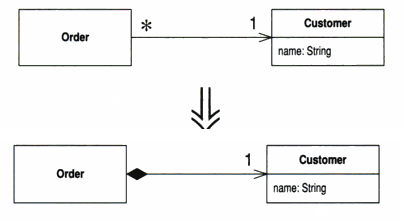
\includegraphics[scale=0.5]{refactoring.png}
  \end{center}
  \caption{Refactoring a reference to a value. Taken from \cite{fowler99refactoring}[pg183].}
  \label{fig:refactoring}
\end{figure}

Before applying the refactoring, each customer may be associated with more than one order. After the refactoring, each customer should be associated with only one order. Fowler indicates that every customer associated with more than one order should be duplicated, such that one customer object exists for each order. Therefore, the migration strategy in Listing \ref{lst:refactoring} is deduced.

Using this process, I deduced migration strategies for each of the refactorings that were applicable to EMF metamodels, and caused inconsistencies between a metamodel and its models. Subsequently, I have recognised some of the metamodel changes in the FPTC project (one of the projects chosen for the co-evolution study) as object-oriented refactorings.

\begin{lstlisting}[caption=Migration strategy for the refactoring in pseudo code., label=lst:refactoring]
for every customer, c
	for every order, o, associated with c
		create a new customer, d
		copy the values of c's attributes into d
	next o
	
	delete c
next c
\end{lstlisting}

Object-oriented refactorings are used to improve the maintainability of existing systems. In other words, they represent only one of the three reasons for evolutionary change defined by \cite{sjoberg93quantifying}. The two other types of changes to object-oriented systems are equally relevant to my research. Consequently, I have obtained further examples of changes made to object-oriented systems from Tim Hoverd, an experienced object-oriented developer. Hoverd's examples include changes made that represent at least one of the other reasons for evolutionary change defined by \cite{sjoberg93quantifying}.

% subparagraph preliminary_study_of_object_oriented_refactorings (end)
% paragraph examples_of_evolution_from_object_oriented_systems (end)


\paragraph{Research collaborations} % (fold)
\label{par:collaborations}
As well as locating example data from object-oriented programs, I am currently collaborating with two colleagues who are using MDE. Adam Sampson, a research assistant at the University of Kent, and I are constructing a metamodel to standardise the way in which his team model process-oriented programs. Heather Barber, a postdoctorate student in the department, and I are investigating the feasibility of implementing a tool for generating story-worlds for interactive narratives.

In both cases, the work involves constructing a metamodel for describing concepts in the domain. The metamodels will be developed incrementally, and consequently will change over time. In both cases, the domain is large, so I am hopeful that evolution will involve more than just additive changes. If so, the data will be used for studying co-evolution.

Both parties have expressed an interest in transforming their models to generate code (possibly via an intermediate model). If realised, the data will be used for studying model synchronisation.

% paragraph collaborations (end)
% subsubsection other_data (end)

\subsubsection{Summary}
To summarise, I have located eight existing MDE projects, three of which contain data that can be analysed to obtain requirements for the development of structures and process for \textbf{co-}evolutionary changes in the context of model-driven engineering. One of the three projects, GMF, will be reserved as a case study for my thesis. Refactorings and other examples from object-oriented programming will supplement the data available from the existing MDE projects. Collaboration with Sampson and Barber will yield further data. Should I discover further sources of model synchronisation, I will expand my research accordingly.




